\chapter{CƠ SỞ LÝ THUYẾT}

\section{Tìm hiểu về Trí tuệ nhân tạo, Học máy, Học sâu}

\subsection{Trí tuệ nhân tạo (Artificial Intelligence - AI)}

Trí tuệ nhân tạo (AI) là một lĩnh vực khoa học tập trung vào việc xây dựng và cải tiến các hệ thống tính toán tự động có thể đảm nhiệm những công việc vốn đòi hỏi trí tuệ của con người. Công nghệ này mô phỏng các quá trình tư duy, học hỏi và giải quyết vấn đề, với mục tiêu xây dựng những hệ thống có khả năng nhận thức, suy nghĩ và hành động một cách tự động.

AI bao gồm nhiều kỹ thuật và phương pháp đa dạng như Học máy (Machine Learning), Xử lý ngôn ngữ tự nhiên (Natural Language Processing) và Thị giác máy tính (Computer Vision). Các tiến bộ kỹ thuật gần đây đóng vai trò then chốt trong việc hiện thực hóa các hệ thống AI hiệu quả và đáng tin cậy cho phép máy tính tiếp thu kiến thức từ dữ liệu, nhận diện các mẫu đặc trưng, thích ứng với hoàn cảnh mới và đưa ra các quyết định một cách thông minh. AI có thể được phân loại thành ba cấp độ:
\begin{itemize}
  \item AI yếu (Narrow AI): AI được phát triển để thực hiện một tác vụ đơn giản, cụ thể, ví dụ như chatbot, hệ thống đề xuất phim, hoặc trợ lý ảo.
  \item AI mạnh (General AI): Có khả năng học và thực hiện bất kỳ nhiệm vụ trí tuệ nào của con người.
  \item AI siêu việt (Super AI): Là giai đoạn lý thuyết trong tương lai, nơi AI có thể vượt xa trí thông minh của con người trong mọi lĩnh vực.
\end{itemize}

Trong thời đại số hóa hiện nay, trí tuệ nhân tạo (AI) ngày càng trở thành yếu tố cốt lõi thúc đẩy sự đổi mới và phát triển trong các ngành như chăm sóc sức khỏe, tài chính, vận tải và ngành công nghiệp giải trí, mang lại những đổi mới đáng kể trong cách chúng ta học tập và làm việc.

\subsection{Học máy (Machine Learning - ML)}

Học máy (Machine Learning) là một phân ngành của Trí tuệ nhân tạo (AI) chuyên nghiên cứu các thuật toán giúp hệ thống học từ dữ liệu và đưa ra quyết định mà không cần mã hóa quy tắc một cách rõ ràng.

Nguyên lý hoạt động của ML dựa trên việc rút ra mô hình từ dữ liệu huấn luyện (training data) để đưa ra dự đoán hoặc quyết định cho dữ liệu mới (dữ liệu kiểm tra).

Học máy bao gồm ba nhóm chính dựa trên cách mô tả tiếp cận dữ liệu:
\begin{itemize}
  \item Học có giám sát (Supervised Learning): Phương pháp này sử dụng tập dữ liệu đã được gán nhãn sẵn để huấn luyện mô hình. Ví dụ việc phân loại thư rác.
  \item Học không giám sát (Unsupervised Learning): Với phương pháp này, hệ thống làm việc với dữ liệu không có nhãn, nhiệm vụ của mô hình là tìm ra những đặc điểm hoặc mối quan hệ tiềm ẩn bên trong. Ví dụ: phân loại người dùng mạng xã hội theo hành vi tương tác.
  \item Học tăng cường (Reinforcement Learning): Dựa trên quá trình tương tác giữa hệ thống và môi trường, trong đó hệ thống nhận được phần thưởng khi thực hiện hành vi đúng. Một minh họa rõ nét là robot học cách di chuyển nhờ việc liên tục thử các ra quyết định và điều chỉnh dựa trên phản hồi môi trường mang lại.
\end{itemize}

\begin{figure}[htbp]
  \centering
  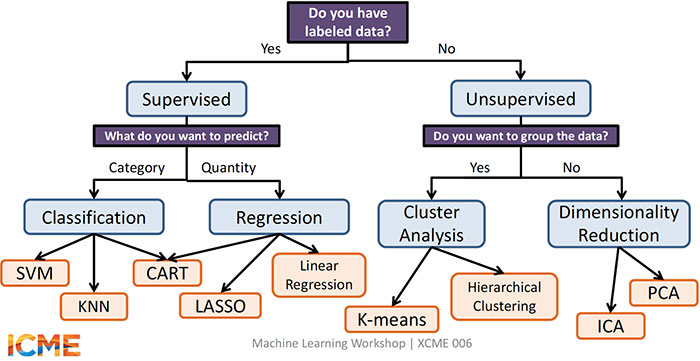
\includegraphics[width=0.8\linewidth]{images/img02.jpeg}
  \caption{Các thuật toán Học máy}
  \label{fig:ml-algorithms}
\end{figure}

\subsection{Học sâu (Deep Learning - DL)}

Học sâu (Deep Learning) là một lĩnh vực trực thuộc học máy, sử dụng các mạng nơ-ron nhiều tầng để xây dựng mô hình toán học dựa trên dữ liệu đầu vào. Deep Learning thường được nhắc đến song song với Trí tuệ nhân tạo (AI) và Dữ liệu lớn (Big Data). Công nghệ này đã được áp dụng và hiện vẫn tiếp tục được ứng dụng rộng rãi trong thực tế, được thúc đẩy mạnh mẽ bởi sự tiến hóa của phần cứng, nhờ vào sức mạnh xử lý của GPU, lượng dữ liệu tăng nhanh, cùng với sự hỗ trợ từ các thư viện như TensorFlow và PyTorch, việc phát triển mô hình đã được đơn giản hóa, giúp cho người dùng dễ dàng thao tác sử dụng hơn.

Học sâu khai thác khả năng học biểu diễn đặc trưng trực tiếp từ dữ liệu. Một quan sát cụ thể, ví dụ hình ảnh, có khả năng được bằng nhiều hình thức khác nhau – từ các vector chứa giá trị điểm ảnh đến các biểu diễn trừu tượng như tập hợp cạnh, vùng hoặc hình khối. Ví dụ minh họa bao gồm nhận diện khuôn mặt hoặc phân tích biểu cảm khuôn mặt. Một điểm mạnh đáng chú ý của học sâu là khả năng loại bỏ các đặc trưng thủ công và thay vào đó là các đặc trưng trích xuất tự động thông qua quá trình học, đặc biệt hiệu quả trong các bài toán học không giám sát (unsupervised learning) và bán giám sát (semi-supervised learning) nhờ vào cấu trúc phân cấp.

Các kiến trúc học sâu tiêu biểu như mạng nơ-ron sâu (Deep Neural Networks - DNN), mạng tích chập (Convolutional Neural Networks - CNN), mạng niềm tin sâu (Deep Belief Networks - DBN) và mạng hồi tiếp (Recurrent Neural Networks - RNN) đã được triển khai rộng rãi trong nhiều lĩnh vực, bao gồm nhận dạng hình ảnh, phân tích giọng nói, xử lý văn bản tự nhiên, âm thanh và sinh học tính toán. Những mô hình này đã chứng minh hiệu quả vượt trội khi giải quyết các tác vụ phức tạp trong thực tiễn.

Thêm vào đó, học sâu hiện nay cũng trở thành một thuật ngữ phổ biến, đôi khi được xem như "thương hiệu" đại diện cho các mạng nơ-ron sâu hiện đại (modern deep neural network).

\begin{figure}[htbp]
  \centering
  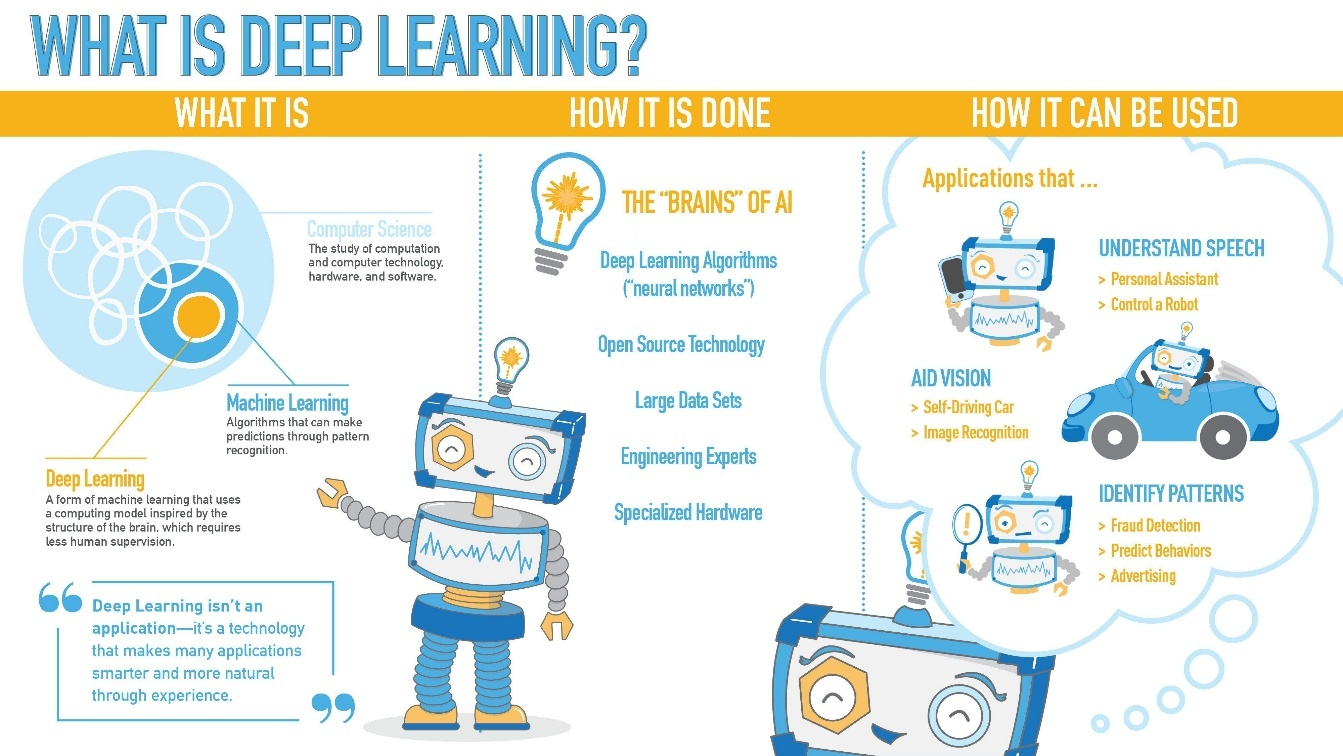
\includegraphics[width=0.8\linewidth]{images/img03.jpeg}
  \caption{Học sâu}
  \label{fig:deep-learning}
\end{figure}

\subsection{Mối quan hệ giữa trí Tuệ nhân tạo, Học máy, Học sâu}

Trí tuệ nhân tạo (Artificial Intelligence – AI), Học máy (Machine Learning – ML) và Học sâu (Deep Learning – DL) là ba khái niệm có mối quan hệ mật thiết với nhau, đồng thời phản ánh tiến trình phát triển tự nhiên của lĩnh vực nghiên cứu về khả năng tiếp nhận kiến thức và tư duy của máy móc.

Trí tuệ nhân tạo là lĩnh vực tổng quát, bao gồm tất cả các phương pháp và kỹ thuật nhằm mục đích tạo ra các hệ thống có khả năng thực hiện các hành vi thông minh tương tự con người. Trong phạm vi này, học máy xuất hiện như một hướng tiếp cận nổi bật, tập trung vào việc xây dựng các kỹ thuật cho phép máy tính có thể học được thông qua dữ liệu mà không cần phải lập trình tường minh cho từng tác vụ cụ thể. Học máy không chỉ giúp tự động hóa quá trình ra quyết định mà còn mở ra khả năng xử lý các vấn đề phức tạp trong môi trường có dữ liệu thay đổi liên tục.

Tiếp nối sự phát triển của học máy, học sâu được xem là một phân nhánh sâu hơn, sử dụng mô hình hệ thống mạng nơ-ron đa tầng (deep neural networks) để mô hình hóa các quan hệ phi tuyến phức tạp giữa dữ liệu đầu vào và đầu ra. Học sâu cho phép khai thác dữ liệu ở quy mô lớn và có khả năng trích xuất đặc trưng tự động, thay vì dựa vào đặc trưng thủ công như trong các phương pháp học máy truyền thống.

Giữa ba lĩnh vực này có mối quan gắn bó chặt chẽ với nhau, được tổ chức theo mô hình lồng ghép – trong đó mỗi lĩnh vực là nền tảng cho lĩnh vực tiếp theo, trong đó học sâu là một phần của học máy, và học máy là một phần của trí tuệ nhân tạo. Cụ thể: Deep Learning $\subset$ Machine Learning $\subset$ Artificial Intelligence. Đây không những là mối quan hệ phân lớp mà còn là sự kế thừa và nâng cao về mặt kỹ thuật và ứng dụng.

\begin{figure}[htbp]
  \centering
  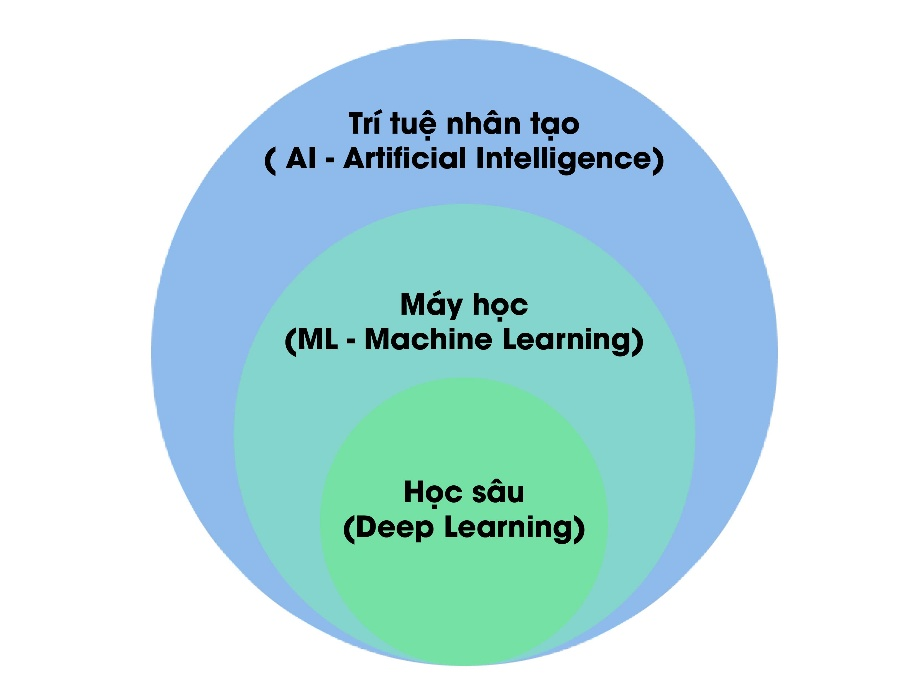
\includegraphics[width=0.8\linewidth]{images/img04.jpeg}
  \caption{Mối quan hệ giữa trí tuệ nhân tạo, học máy, học sâu}
  \label{fig:ai-ml-dl}
\end{figure}

\section{Các thành phần cơ bản trong hệ thống học máy và học sâu}

\subsection{Dữ liệu trong học máy và học sâu}

Dữ liệu là yếu tố cốt lõi trong suốt quá trình đào tạo mô hình học máy và học sâu. Chất lượng và số lượng dữ liệu ảnh hưởng trực tiếp đến độ tin cậy và khả năng mở rộng của mô hình.

Phân loại dữ liệu:
\begin{itemize}
  \item Dữ liệu có cấu trúc (Structured data): Dữ liệu dạng bảng, có trường và giá trị rõ ràng, như cơ sở dữ liệu SQL.
  \item Dữ liệu phi cấu trúc (Unstructured data): Hình ảnh, video, âm thanh, văn bản...
  \item Dữ liệu bán cấu trúc (Semi-structured data): JSON, XML hoặc log hệ thống.
\end{itemize}

Tiền xử lý dữ liệu (Data Preprocessing): Là bước quan trọng để loại bỏ nhiễu, chuẩn hóa đầu vào, và tăng độ chính xác cho mô hình. Bao gồm:
\begin{itemize}
  \item Làm sạch dữ liệu (loại bỏ nhiễu trong tập dữ liệu thông qua việc xử lý thiếu hụt thông tin và phát hiện ngoại lệ),
  \item Chuẩn hóa (Normalization, Standardization),
  \item Mã hóa dữ liệu (One-hot, Label encoding),
  \item Chia tập dữ liệu (train/test/validation),
  \item Tăng cường dữ liệu (Data Augmentation – với hình ảnh hoặc âm thanh).
\end{itemize}

\subsection{Kiến trúc mạng nơ-ron nhân tạo}

Mạng nơ-ron nhân tạo (ANN) là thành phần chính trong học sâu. Cấu trúc cơ bản của một mạng gồm ba lớp~\cite{zhangMultilayerPerceptrons}:
\begin{itemize}
  \item Lớp đầu vào (Input layer): Nhận dữ liệu thô từ bên ngoài.
  \item Lớp ẩn (Hidden layer): Thực hiện các phép toán, phát hiện đặc trưng.
  \item Lớp đầu ra (Output layer): Trả kết quả dự đoán cuối cùng.
\end{itemize}

Các nơ-ron trong từng lớp được kết nối với các nơ-ron ở lớp kế tiếp thông qua trọng số. Việc sử dụng nhiều lớp ẩn trong các mạng học sâu giúp mô hình học được những đặc trưng dữ liệu ở mức độ trừu tượng cao hơn.

\begin{figure}[htbp]
  \centering
  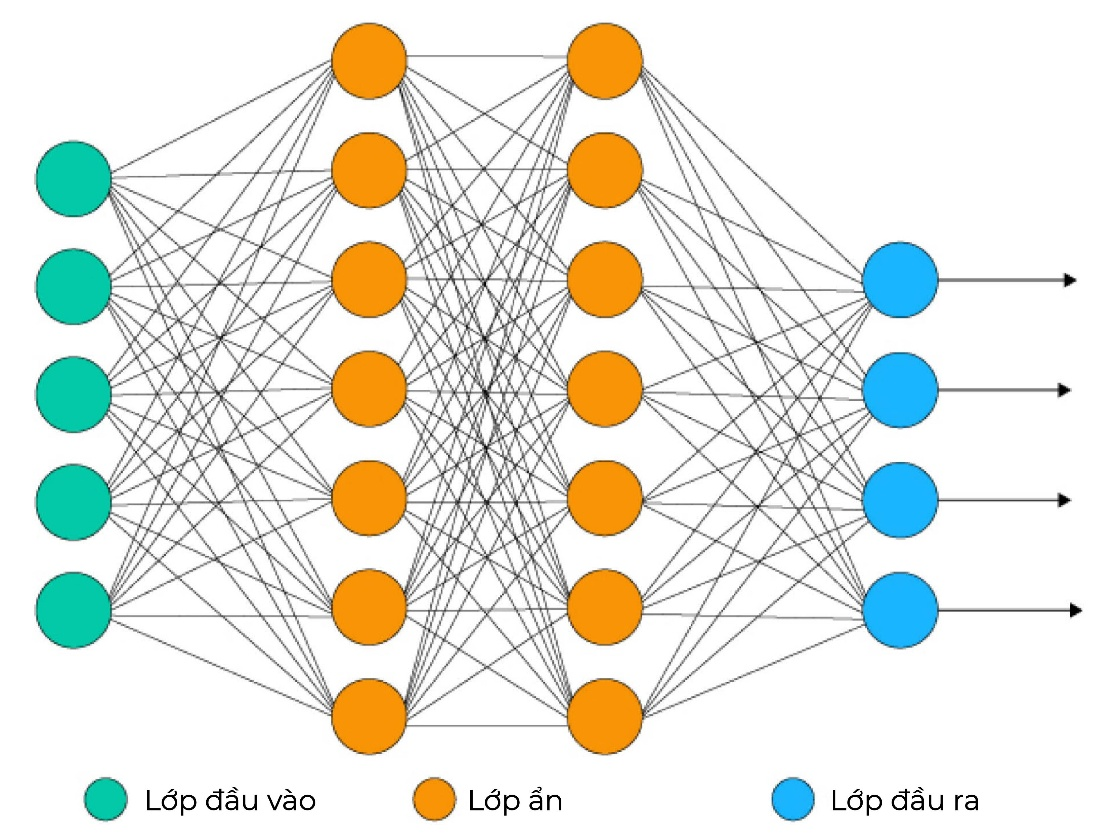
\includegraphics[width=0.8\linewidth]{images/img05.jpeg}
  \caption{Cấu trúc mạng nơ-ron nhân tạo}
  \label{fig:ann}
\end{figure}

Một số kiến trúc đặc biệt:
\begin{itemize}
  \item CNN (Mạng tích chập): Xử lý ảnh và nhận diện không gian.
  \item RNN và LSTM: Phù hợp với dữ liệu chuỗi (speech, text).
  \item Transformer: Mô hình học ngữ cảnh sâu và xử lý song song trong NLP.
  \item Autoencoder: Dùng để giảm chiều dữ liệu, trích xuất đặc trưng.
\end{itemize}

\subsection{Quá trình huấn luyện mô hình}

Huấn luyện mô hình là quá trình tối ưu trọng số sao cho độ lệch giữa kết quả mô hình dự đoán và giá trị thực tế là nhỏ nhất~\cite{pytorchOptimizingModelParameters}. Gồm các bước:
\begin{enumerate}
  \item Khởi tạo trọng số (Weight Initialization)
  \item Lan truyền tiến (Forward Propagation)
  \item Tính toán sai số (Loss Function): Các hàm như MSE, Cross-Entropy.
  \item Lan truyền ngược (Backpropagation): Cập nhật trọng số theo hướng giảm sai số.
  \item Tối ưu hóa (Optimization): Dùng các thuật toán như SGD, Adam, RMSProp.
  \item Chống overfitting~\cite{zhangGeneralization}: Dropout, Regularization (L1/L2), Early Stopping, v.v.
\end{enumerate}

\subsection{Đánh giá mô hình}

Quy trình đánh giá mô hình giúp xác định độ chính xác và tính tổng quát hóa~\cite{zhangGeneralization}. Một số chỉ số phổ biến:
\begin{itemize}
  \item Độ chính xác (Accuracy)
  \item Precision / Recall / F1-Score
  \item AUC-ROC (cho mô hình phân loại)
  \item MAE, RMSE (cho bài toán hồi quy)
\end{itemize}
Công cụ hỗ trợ đánh giá: confusion matrix, learning curve, validation curve,\ldots

\subsection{Các công cụ và thư viện hỗ trợ}

Triển khai các giải pháp dựa trên học máy và học sâu hiện nay được hỗ trợ bởi rất nhiều thư viện mã nguồn mở mạnh mẽ~\cite{tensorflowTensorFlow,pytorchOptimizingModelParameters,scikit-learnMachineLearning,numpyNumPy,matplotlibVisualizationPython}:

\begin{table}[htbp]
  \centering
  \caption{Các công cụ, thư viện hỗ trợ}
  \label{tab:tools}
  \begin{tabular}{@{}l l l@{}}
    \toprule
    Công cụ/Thư viện & Mục đích & Ngôn ngữ \\
    \midrule
    TensorFlow & Học sâu, hỗ trợ GPU, mô hình hóa linh hoạt & Python, C++ \\
    Keras & API cấp cao của TensorFlow, dễ dùng & Python \\
    PyTorch & Mạnh mẽ và linh hoạt, phổ biến trong nghiên cứu & Python \\
    OpenCV & Xử lý ảnh, phát hiện đối tượng & Python, C++ \\
    Pandas, NumPy & Xử lý dữ liệu & Python \\
    \bottomrule
  \end{tabular}
\end{table}

\section{Ứng dụng của trí tuệ nhân tạo, học máy và học sâu}

Cùng với sự phát triển nhanh chóng của phần cứng và dữ liệu lớn (Big Data), AI, học máy và học sâu đã và đang được ứng dụng mạnh mẽ trong nhiều ngành nghề, góp phần nâng cao năng suất, tối ưu hóa vận hành, và đóng góp vào việc tạo dựng giá trị thiết thực cho doanh nghiệp cũng như xã hội.

\subsection{Thị giác máy tính (Computer Vision)}

Thị giác máy tính là một trong những lĩnh vực cốt lõi của trí tuệ nhân tạo, cho phép máy móc có khả năng nhận diện và hiểu biết về môi trường xung quanh qua các hình ảnh hoặc đoạn video. Công nghệ này sử dụng ứng dụng các phương pháp học máy, trong đó học sâu đóng vai trò then chốt, vốn nổi bật trong việc xử lý các hình ảnh có cấu trúc phức tạp và đa dạng về đặc trưng.

Một trong những ứng dụng rộng rãi là hệ thống nhận dạng khuôn mặt, sử dụng mạng nơ-ron tích chập (CNN) để phân tích các đặc trưng khuôn mặt, áp dụng rộng rãi trong mở khóa thiết bị di động, hệ thống giám sát an ninh, hay quản lý điểm danh thông minh.

Trong lĩnh vực y tế, học sâu được dùng để phân loại hình ảnh y học như ảnh CT, MRI, X-quang nhằm phát hiện bệnh lý như ung thư, xuất huyết hoặc tổn thương mô mềm. Các hệ thống này không chỉ hỗ trợ bác sĩ mà còn nâng cao độ chính xác chẩn đoán nhờ khả năng học từ hàng triệu mẫu ảnh.

Công nghệ phát hiện và theo dõi đối tượng cũng là một bước tiến lớn, ứng dụng trong xe tự hành và các hệ thống giám sát giao thông thông minh. Thuật toán như YOLO, SSD hay Mask R-CNN có khả năng nhận diện nhiều đối tượng trong thời gian thực, hỗ trợ các hệ thống đưa ra quyết định điều hướng và phản ứng kịp thời.

Thị giác máy tính cũng góp phần trong việc số hóa tài liệu thông qua công nghệ nhận diện ký tự quang học (OCR), giúp máy đọc được văn bản từ ảnh chụp, hóa đơn hoặc tài liệu scan, hỗ trợ hiệu quả trong lưu trữ và tìm kiếm thông tin.

Ngoài ra, trong lĩnh vực sáng tạo và giải trí, thị giác máy tính được tích hợp công nghệ AR vào việc xử lý và áp dụng hiệu ứng khuôn mặt trực tiếp, hiệu ứng video, hoặc thậm chí trong các công cụ tạo nghệ thuật số nhờ khả năng hiểu cấu trúc và thành phần hình ảnh.

\begin{figure}[htbp]
  \centering
  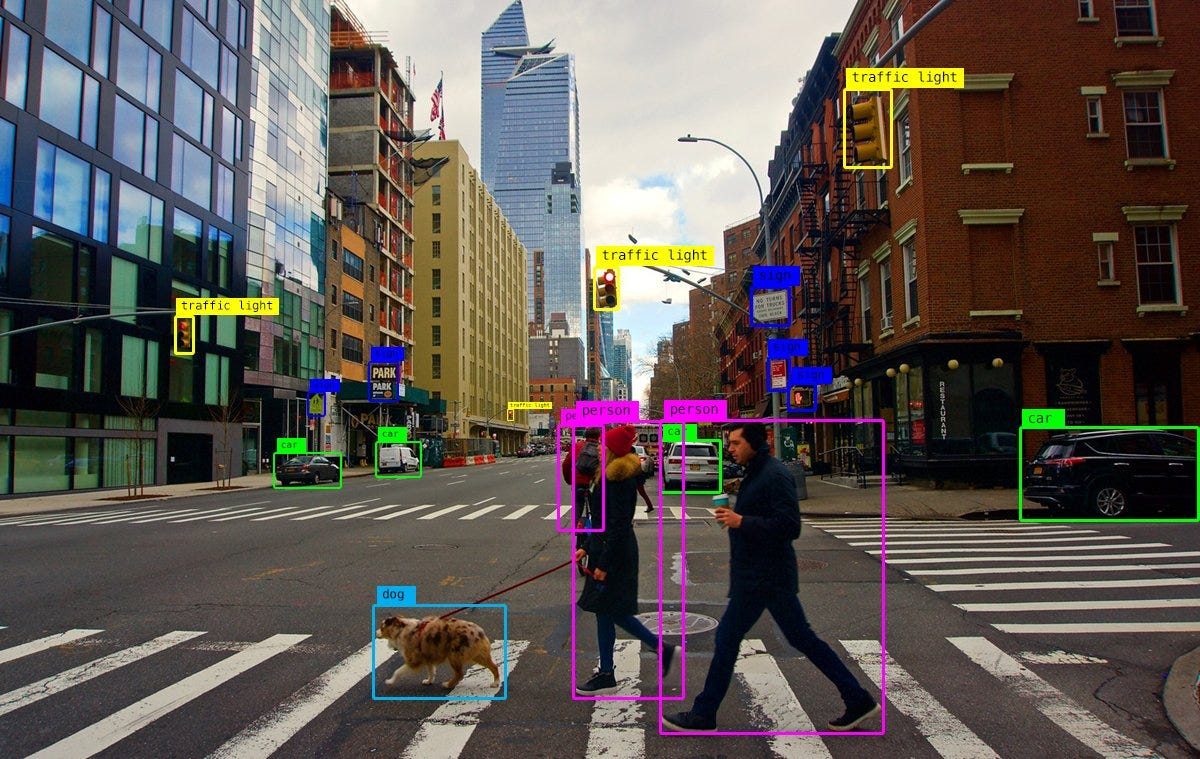
\includegraphics[width=0.8\linewidth]{images/img06.jpg}
  \caption{Ứng dụng của Thị giác máy tính trong nhận diện vật thể}
  \label{fig:cv-detection}
\end{figure}

\subsection{Xử lý ngôn ngữ tự nhiên (Natural Language Processing - NLP)}

Xử lý ngôn ngữ tự nhiên là một lĩnh vực nghiên cứu nhằm trang bị cho máy tính khả năng hiểu, phân tích và sinh ngôn ngữ tự nhiên theo cách mà con người sử dụng trong giao tiếp. Đây là một trong những hướng phát triển sôi động nhất của AI hiện đại, với sự bùng nổ mạnh mẽ của các mô hình học sâu như BERT, GPT, T5 và các mô hình ngôn ngữ lớn (LLMs).

Một trong những ví dụ điển hình nhất của NLP là chatbot và trợ lý ảo – như Siri, Alexa, Google Assistant – cho phép máy có thể hiểu các yêu cầu bằng giọng nói hoặc văn bản và phản hồi một cách tự nhiên. Học sâu đóng vai trò quan trọng trong việc tạo ra phản hồi mạch lạc, đúng ngữ cảnh và có khả năng cá nhân hóa cao.

Dịch máy tự động cũng đã có bước tiến vượt bậc. Các mô hình học sâu tiên tiến như Transformer đã mở ra nhiều hướng tiếp cận hiệu quả, hệ thống như Google Translate hay DeepL không chỉ dịch chính xác hơn mà còn giữ được ngữ điệu và phong cách văn bản gốc.

Phân tích cảm xúc là một ứng dụng khác, sử dụng NLP để đánh giá tâm trạng hoặc thái độ của người dùng dựa trên nội dung văn bản – rất hữu ích trong phân tích đánh giá sản phẩm, phản hồi khách hàng hoặc theo dõi dư luận trên mạng xã hội.

Trong lĩnh vực tóm tắt văn bản, các mô hình hiện đại có thể tự động rút gọn nội dung từ bài viết, tài liệu dài thành bản tóm tắt ngắn gọn, vẫn đảm bảo thông tin cốt lõi, phục vụ cho nghiên cứu, báo cáo hay tổng hợp tin tức.

Ngoài ra, NLP hỗ trợ nhận diện các thực thể tên riêng thông qua kỹ thuật NER, cho phép trích xuất thông tin quan trọng như tên người, địa điểm, tổ chức từ văn bản – một phương pháp hiệu quả trong lĩnh vực phân tích dữ liệu văn bản và xây dựng cơ sở tri thức.

Nhờ sự phát triển đồng bộ của AI, học máy và học sâu, NLP ngày càng trở nên mạnh mẽ, không chỉ giúp máy hiểu ngôn ngữ con người mà còn có khả năng tham gia đối thoại tự nhiên, sinh văn bản sáng tạo và hỗ trợ nhiều tác vụ trí tuệ phức tạp.

\begin{figure}[htbp]
  \centering
  
\includegraphics[width=0.8\linewidth]{images/img07.png}
  \caption{Chatbot – Ứng dụng của xử lý ngôn ngữ tự nhiên}
  \label{fig:chatbot}
\end{figure}

\subsection{Xử lý ảnh}

Xử lý ảnh là một trong những bài toán nền tảng trong trí tuệ nhân tạo, học máy và học sâu, với mục tiêu chính là phân tích, trích xuất thông tin từ hình ảnh hoặc thực hiện các phép biến đổi nhằm phục vụ cho những tác vụ cao hơn như nhận diện, theo dõi, hoặc ra quyết định.

Một ứng dụng quen thuộc là gắn thẻ hình ảnh (image tagging), chẳng hạn như khi người dùng đăng ảnh lên mạng xã hội, thuật toán có khả năng nhận diện tự động và đề xuất thẻ tên cho khuôn mặt xuất hiện trong ảnh. Cơ chế đằng sau đó thường dựa vào các mô hình học sâu, trong đó mạng nơ-ron CNN được sử dụng phổ biến nhất, có khả năng học từ dữ liệu gắn nhãn sẵn (ảnh người dùng từng được gắn thẻ trước đó), từ đó nhận diện lại trong các bức ảnh mới.

Một ứng dụng khác là nhận dạng ký tự quang học (OCR – Optical Character Recognition), cho phép chuyển đổi hình ảnh chứa văn bản thành dữ liệu số có thể chỉnh sửa và tìm kiếm. Các mô hình học máy và học sâu được phát triển nhằm mục đích nhận dạng các ký tự xuất hiện trong hình ảnh, bất kể font chữ, bố cục hay chất lượng hình ảnh, từ đó phục vụ cho số hóa tài liệu, trích xuất thông tin trên hóa đơn, văn bản hành chính\ldots

Trong lĩnh vực phương tiện tự hành, xử lý ảnh đóng vai trò như “đôi mắt” của hệ thống điều khiển. Thuật toán học máy và học sâu liên tục xử lý các khung hình thu được từ camera gắn trên xe, giúp phát hiện mép đường, biển báo, làn xe, người đi bộ và các vật cản. Đây là tiền đề để xe đưa ra hành động như rẽ, phanh hay tăng tốc một cách chính xác và an toàn.

\subsection{Y tế và chăm sóc sức khỏe}

Trong lĩnh vực y tế, trí tuệ nhân tạo đóng vai trò quan trọng trong việc hỗ trợ bác sĩ chẩn đoán và ra quyết định điều trị. Học máy được áp dụng để nghiên cứu trong hồ sơ bệnh án số (EHR), từ đó phát hiện sớm nguy cơ mắc bệnh như tiểu đường, tim mạch, hoặc tái phát ung thư. Học sâu trong xử lý hình ảnh y tế còn đặc biệt hiệu quả như X-quang, CT hay MRI góp phần hỗ trợ phát hiện sớm tổn thương, khối u với độ chính xác cao hơn cả một số chuyên gia trong từng tình huống cụ thể.

Ngoài ra, các thuật toán AI còn góp phần thúc đẩy quá trình nghiên cứu và phát triển dược phẩm, mô phỏng phản ứng phân tử và tối ưu hiệu năng thử nghiệm lâm sàng. Các hệ thống khuyến nghị điều trị, kết hợp dữ liệu bệnh nhân và hướng dẫn y khoa, là sự tổng hòa giữa AI truyền thống và các mô hình học máy hiện đại.

\subsection{Tài chính – ngân hàng}

AI, ML và DL đang làm thay đổi sâu sắc ngành tài chính. Các mô hình học máy hỗ trợ quy trình chấm điểm tín dụng, tự động hóa quy trình phân tích rủi ro tiềm ẩn cùng với nhận dạng các hành vi lừa đảo trong giao dịch tài chính nhờ vào việc học từ dữ liệu lịch sử. Học sâu còn được triển khai trong việc phân tích chuỗi thời gian phức tạp như biến động thị trường chứng khoán hoặc hành vi khách hàng đa kênh.

Ngoài ra, các tổ chức tài chính, bao gồm ngân hàng đã ứng dụng chatbot thông minh dựa trên học sâu để cung cấp tư vấn tài chính cá nhân hóa, giúp cải thiện trải nghiệm khách hàng và giảm tải cho tổng đài viên. Từ đó, AI không chỉ hỗ trợ tự động hóa, mà còn tạo ra lợi thế cạnh tranh vượt trội trong thị trường tài chính hiện đại.

\subsection{Giao thông và phương tiện tự hành}

Phương tiện tự lái là một minh chứng rõ ràng cho việc triển khai sâu rộng các giải pháp trí tuệ nhân tạo trong thực tiễn của cả AI, ML và DL. AI giúp hệ thống đưa ra quyết định tổng thể, trong khi ML học từ hành vi lái xe để tối ưu hoá hành động, và DL xử lý trực tiếp tín hiệu đầu vào từ camera, radar, LiDAR để nhận diện đường đi, vật cản, biển báo hoạt động theo thời gian thực.

Giải pháp quản lý giao thông hiện đại và thông minh dựa trên bản đồ số cũng ứng dụng học máy nhằm xử lý và khai thác dữ liệu lớn trong thời gian thực, từ đó hỗ trợ quá trình ra quyết định hiệu quả hơn, tối ưu hóa lộ trình. Ở cấp đô thị, AI giúp phân tích dòng xe, dự báo mật độ giao thông, điều phối đèn tín hiệu một cách thích ứng, góp phần giảm tắc nghẽn và tai nạn.

\subsection{Công nghiệp và sản xuất}

Trong công nghiệp, AI giúp cải thiện hiệu suất và giảm thiểu lãng phí thông qua các hệ thống ra quyết định thông minh. Học máy được ứng dụng trong bảo trì dự đoán – nơi các mô hình học từ dữ liệu cảm biến để dự báo tình trạng máy móc, tránh hỏng hóc đột xuất. Học sâu hỗ trợ thị giác máy tính trong dây chuyền kiểm tra chất lượng tự động hóa, giúp hệ thống phát hiện lỗi sản phẩm với tốc độ và độ chính xác cao.

Ngoài ra, robot cộng tác (cobots) – thường được điều khiển bởi hệ thống học sâu – có khả năng học hỏi từ hành vi con người và làm việc linh hoạt trong môi trường sản xuất hỗn hợp. Việc tối ưu chuỗi cung ứng cũng dựa vào các mô hình học máy để phân tích xu hướng tiêu dùng, dự báo nhu cầu và quản lý kho hiệu quả hơn.

\subsection{Giáo dục và đào tạo}

AI hỗ trợ cá nhân hóa quá trình học tập bằng cách đề xuất nội dung phù hợp với trình độ và sở thích của từng học sinh. Học máy được ứng dụng trong việc nghiên cứu hành vi học tập và dự đoán nguy cơ bỏ học hoặc tụt lùi trong quá trình học, từ đó hỗ trợ giảng viên đưa ra các can thiệp kịp thời.

Học sâu giữ vai trò thiết yếu trong việc xây dựng các hệ thống chấm điểm tự động, đặc biệt là với bài tập lập trình hoặc xử lý ngôn ngữ tự nhiên. Thêm vào đó, công nghệ thực tế ảo (VR/AR) kết hợp với AI mở ra các mô hình đào tạo mới, mô phỏng tình huống phức tạp như thí nghiệm hóa học, mô phỏng phòng mổ hay huấn luyện kỹ năng mềm.

\section{Tiểu kết chương 1}

Trong chương này, chúng ta đã cùng nhau tìm hiểu tổng quan về ba lĩnh vực công nghệ nổi bật và có ảnh hưởng lớn trong kỷ nguyên số hiện nay là trí tuệ nhân tạo (AI), học máy (Machine Learning) và học sâu (Deep Learning). Trong đó, AI là khái niệm tổng thể, còn học máy và học sâu đóng vai trò là những phương pháp then chốt trong việc phát triển các hệ thống thông minh giúp cho máy tính khai thác dữ liệu để tự động rút ra kết luận và có khả năng tự đưa ra quyết định dựa trên dữ liệu đầu vào mà không phụ thuộc vào các quy tắc được lập trình sẵn.

Chương còn đi sâu tìm hiểu các yếu tố thiết yếu trong một hệ thống học máy, bắt đầu từ dữ liệu đầu vào, mô hình mạng nơ-ron nhân tạo, quy trình huấn luyện và đánh giá mô hình, cùng với các công cụ hỗ trợ phổ biến như TensorFlow, PyTorch, Scikit-learn,\ldots Những kiến thức này đóng vai trò nền tảng trong việc phát triển các hệ thống thông minh ứng dụng trong thực tế.

Ngoài ra, chương cũng trình bày một số ứng dụng tiêu biểu của AI và học sâu trong nhiều lĩnh vực khác nhau. Những ví dụ này cho thấy rõ ràng tính thực tiễn cũng như tác động mạnh mẽ của các công nghệ đối với cuộc sống của con người.

Những nội dung đã giới thiệu trong chương 1 sẽ là cơ sở lý thuyết quan trọng, hỗ trợ cho việc khai thác sâu hơn ở các chương sau, nơi chúng ta nhắm đến mục tiêu giải quyết bài toán đặc thù mà đề tài hướng đến, lựa chọn mô hình học sâu phù hợp, cũng như các bước triển khai, huấn luyện và đánh giá mô hình trong thực tiễn.
